\chapter{Introduction}
\label{chap:intro}

%\hspace{0.7cm}
%\IEEEPARstart{I}{n}
\hspace{0.7cm}
Write down your introduction here. This is the first paragraph. Penulisan introduction dapat mulai dilakukan dari sini. Ini merupakan paragraf pertama.

\vfill
Paragraph 2 is here. Write down $\backslash cite\{nameofref1\}$ (example: \cite{nameofref1}) to cite any reference taken from the citation you have included by using syntax $\backslash bibliography\{mybib\}$ below, where $mybib$ is a file originally named as $mybib.bib$ with $bibtex$ extension. Paragraf 2 disini. Tuliskan $\backslash cite\{nameofref1\}$ (contoh: \cite{nameofref1}) untuk mereferensi salah satu dari kumpulan referensi yang diambil dari syntax $\backslash bibliography\{mybib\}$ dibawah. $mybib$ sendiri merupakan nama file $mybib.bib$ yang dimasukkan diakhir paper ini. 

\vfill
For a multiple citation call, you can use \url{\cite{nameofref1, nameofref2}} (example: \cite{nameofref1, nameofref2}) and it will cite multiple references for you. Fell free to try it by yourself. Untuk pemanggilan citation lebih dari satu dalam satu kali panggilan, anda dapat menggunakan syntax \url{\cite{nameofref1, nameofref2}} (contoh: \cite{nameofref1, nameofref2}). Silahkan anda coba sendiri untuk prakteknya.

%
%\begin{figure*}
%  \centering
%   \begin{subfigure}[b]{0.48\textwidth}
%       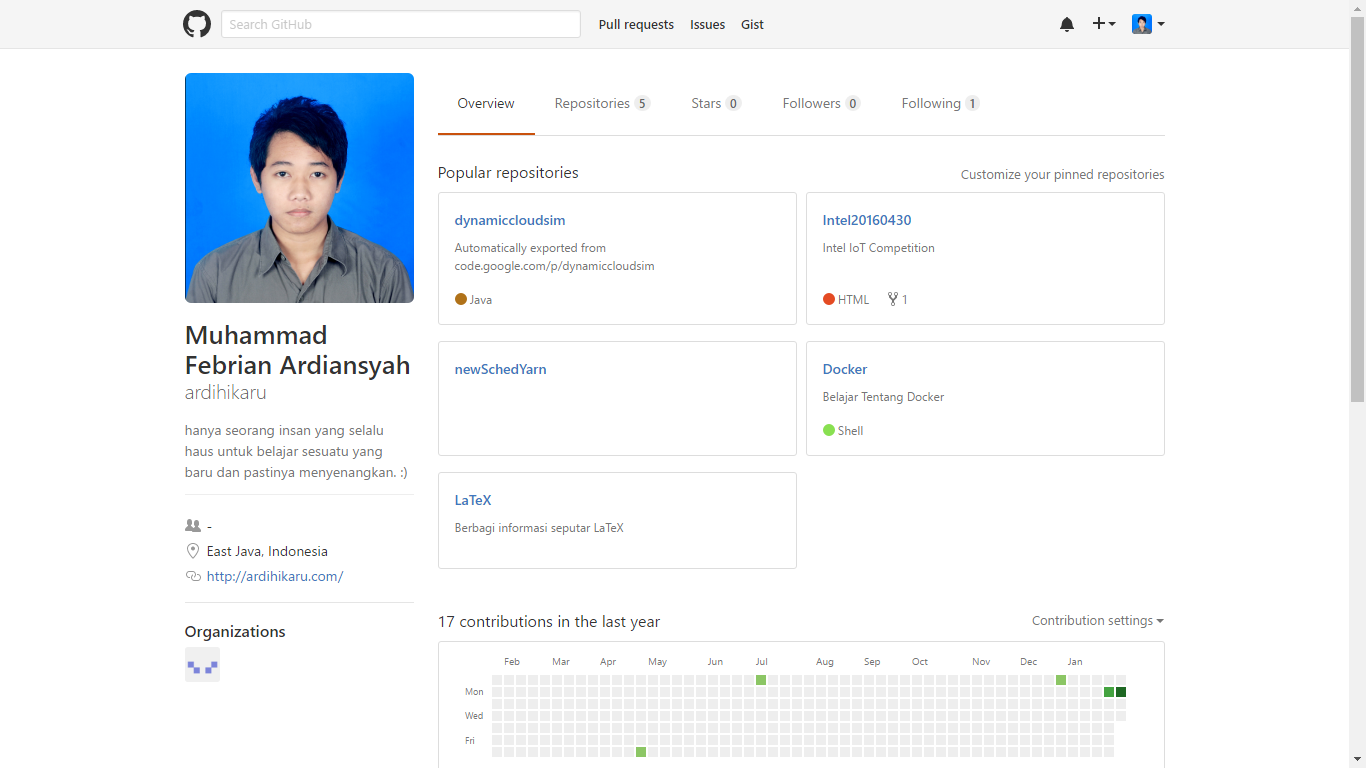
\includegraphics[width=\textwidth, keepaspectratio]{github}
%       \caption{Food choosing}
%       \label{fig:fig1a}
%   \end{subfigure}
%   \begin{subfigure}[b]{0.48\textwidth}
%       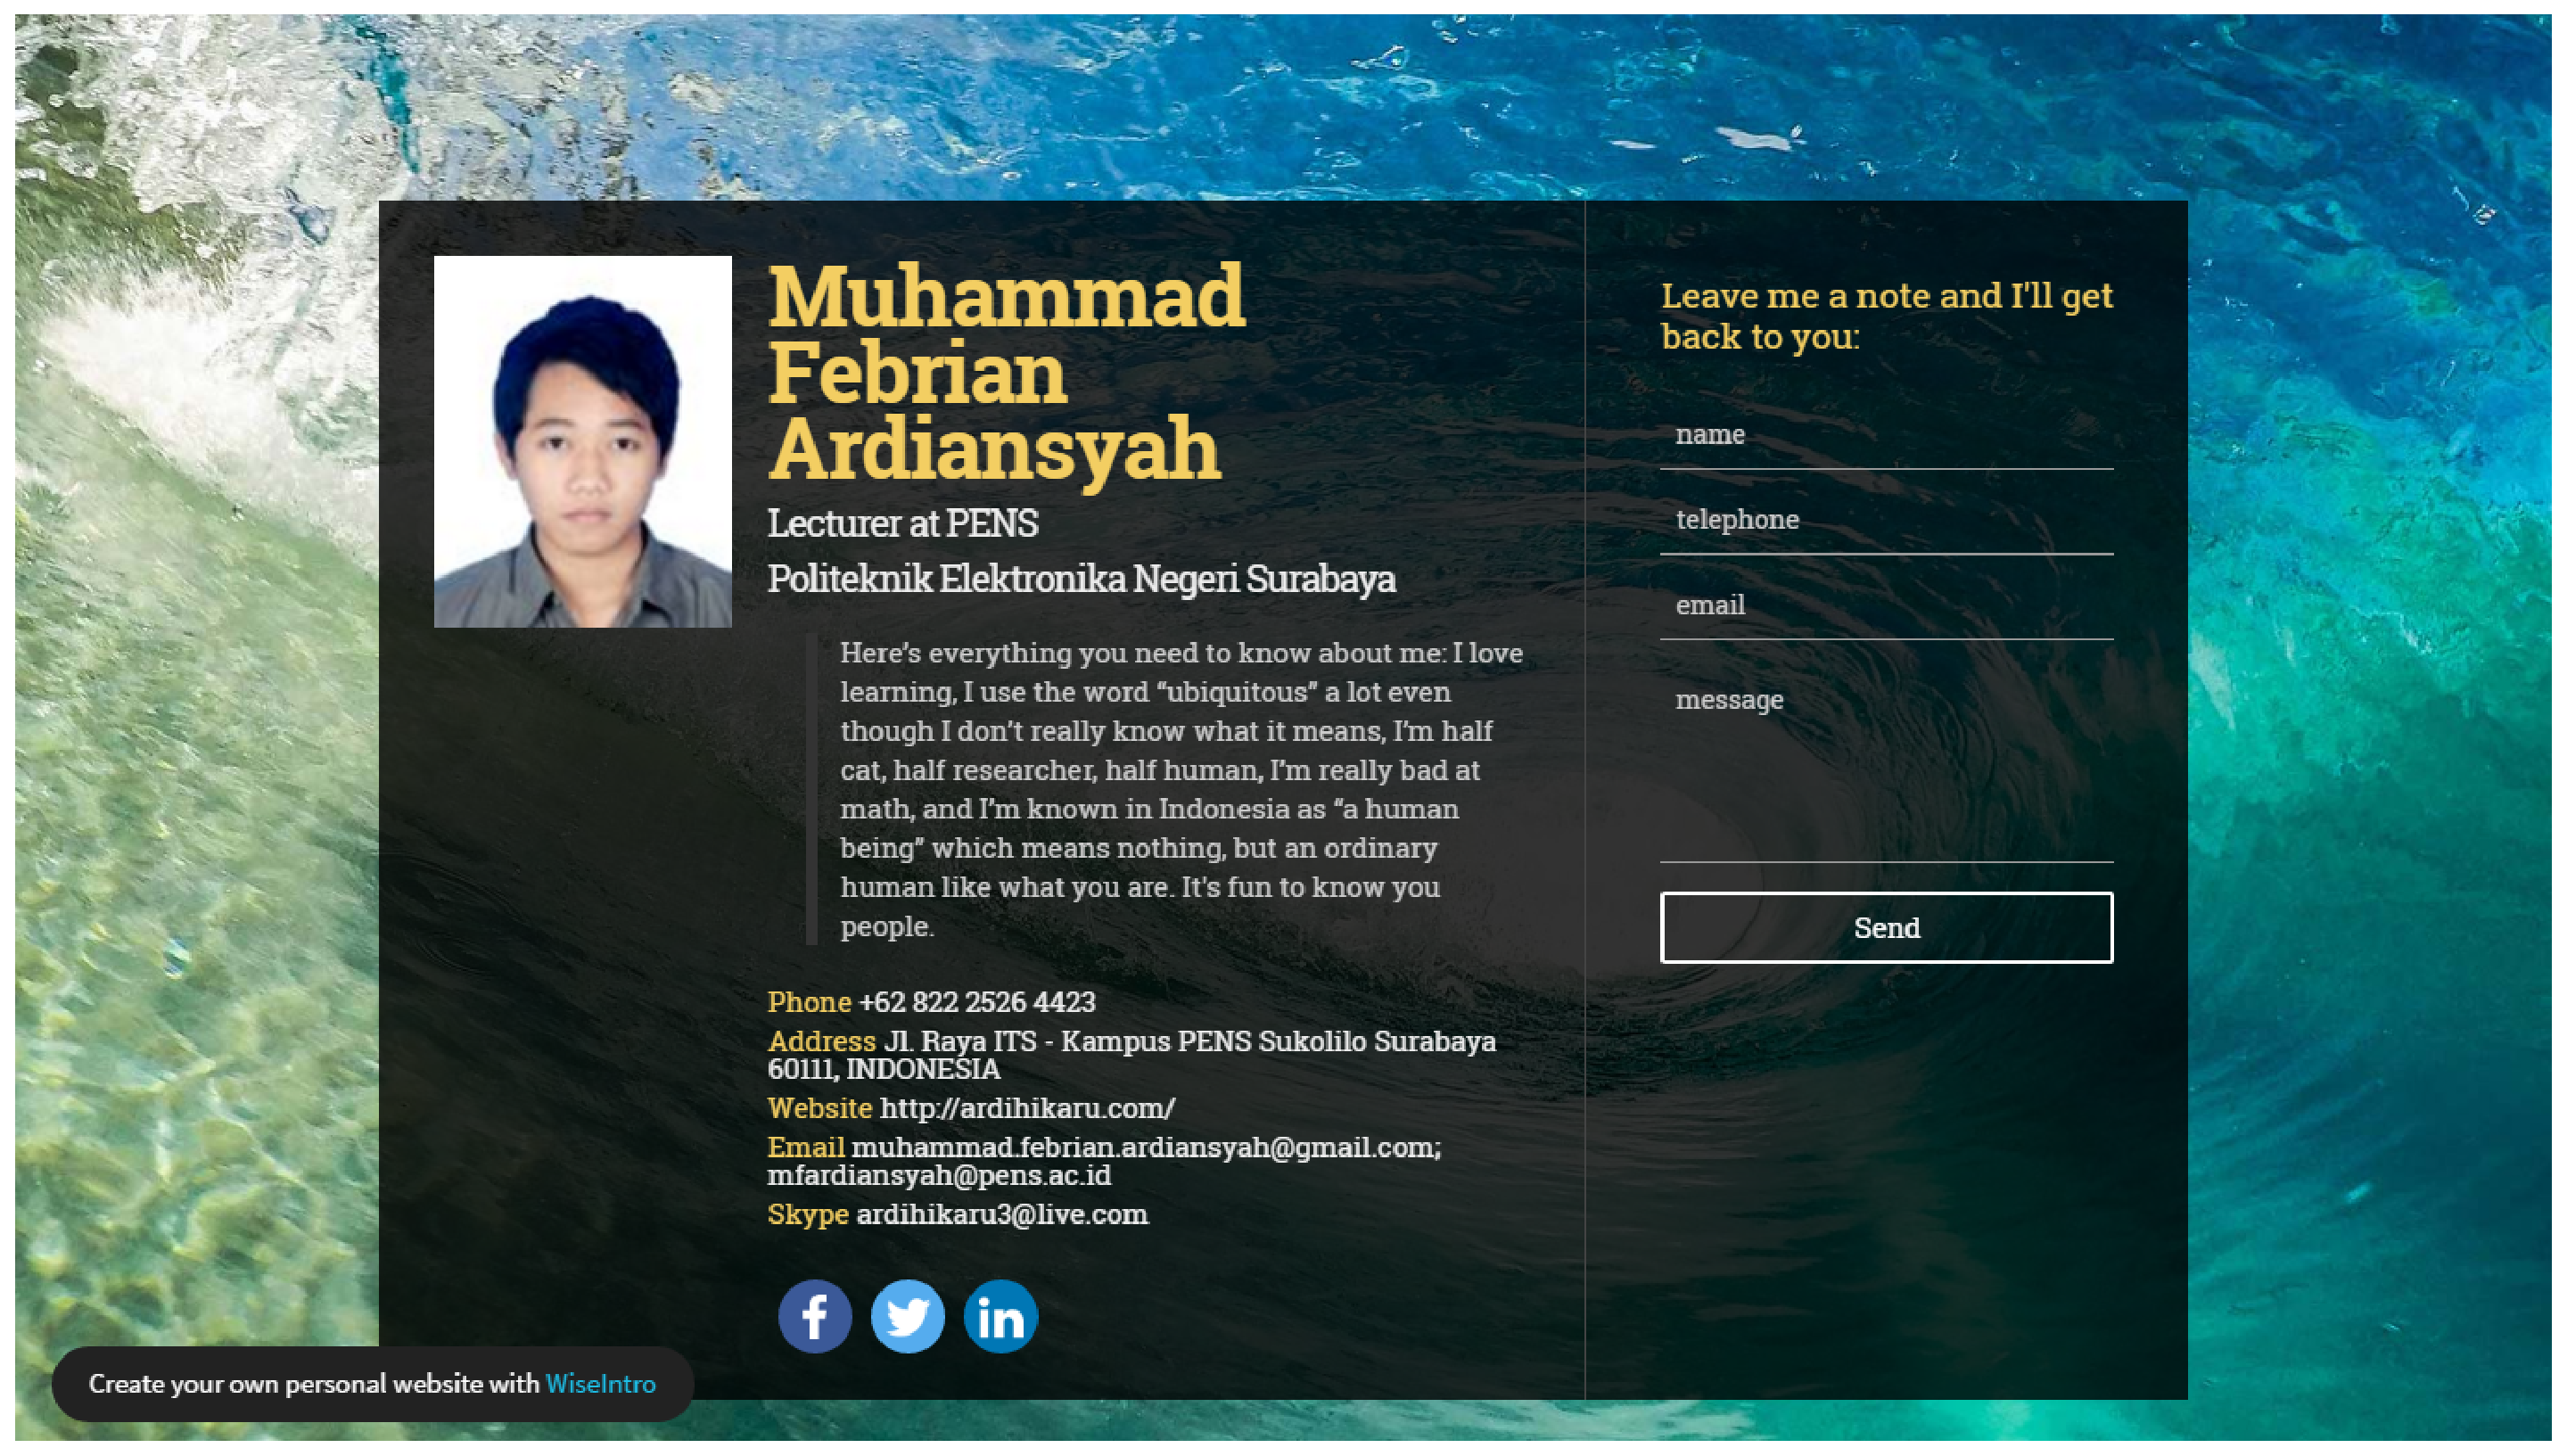
\includegraphics[width=\textwidth, keepaspectratio]{intro}
%       \caption{Interrelationship of different factors for different consumers}
%       \label{fig:fig1b}
%   \end{subfigure}
%   \caption{The difficulties of choosing food and its different adverse reactions}\label{fig1}
%\end{figure*}
%

\begin{figure}[H]
\centering
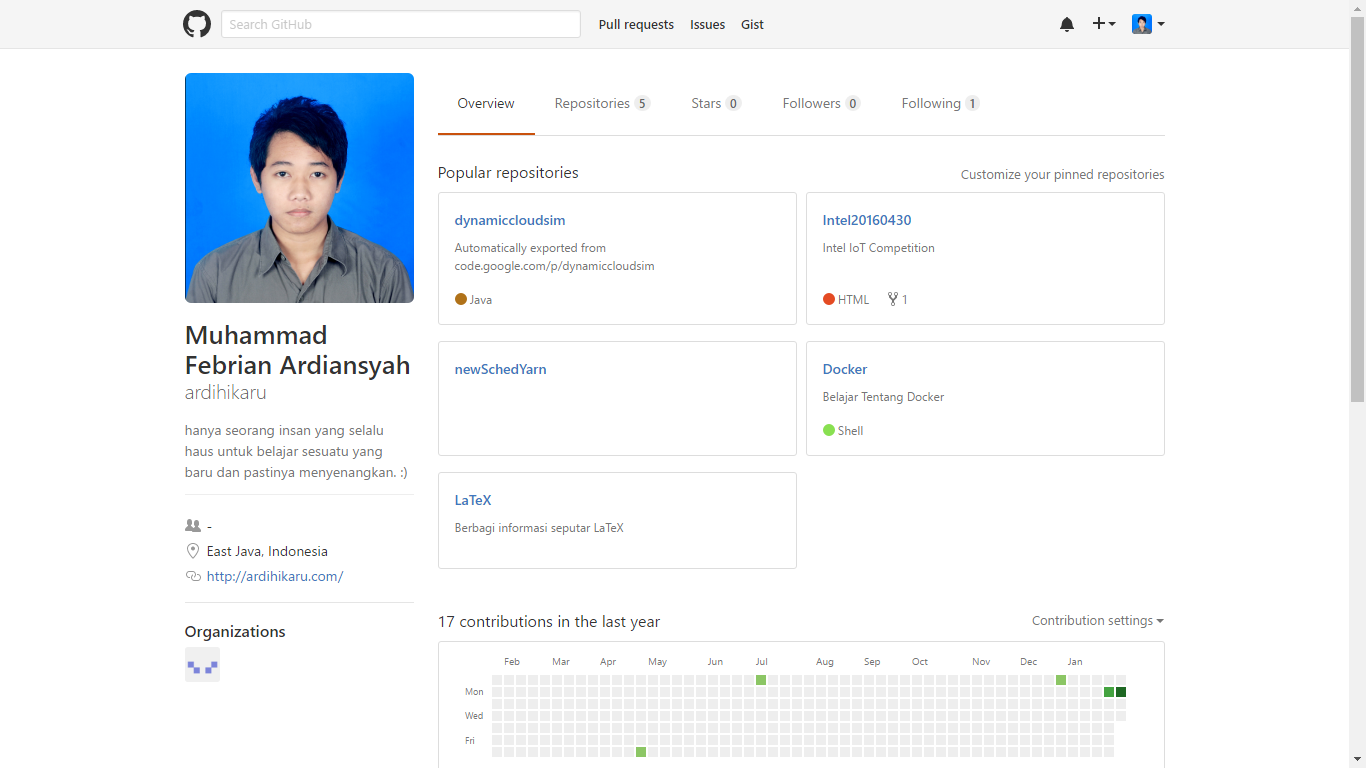
\includegraphics[width=120mm, height=120mm, keepaspectratio]{github}
\caption{Intro}
\label{fig:fig1a}
\end{figure}

\begin{figure}[H]
\centering
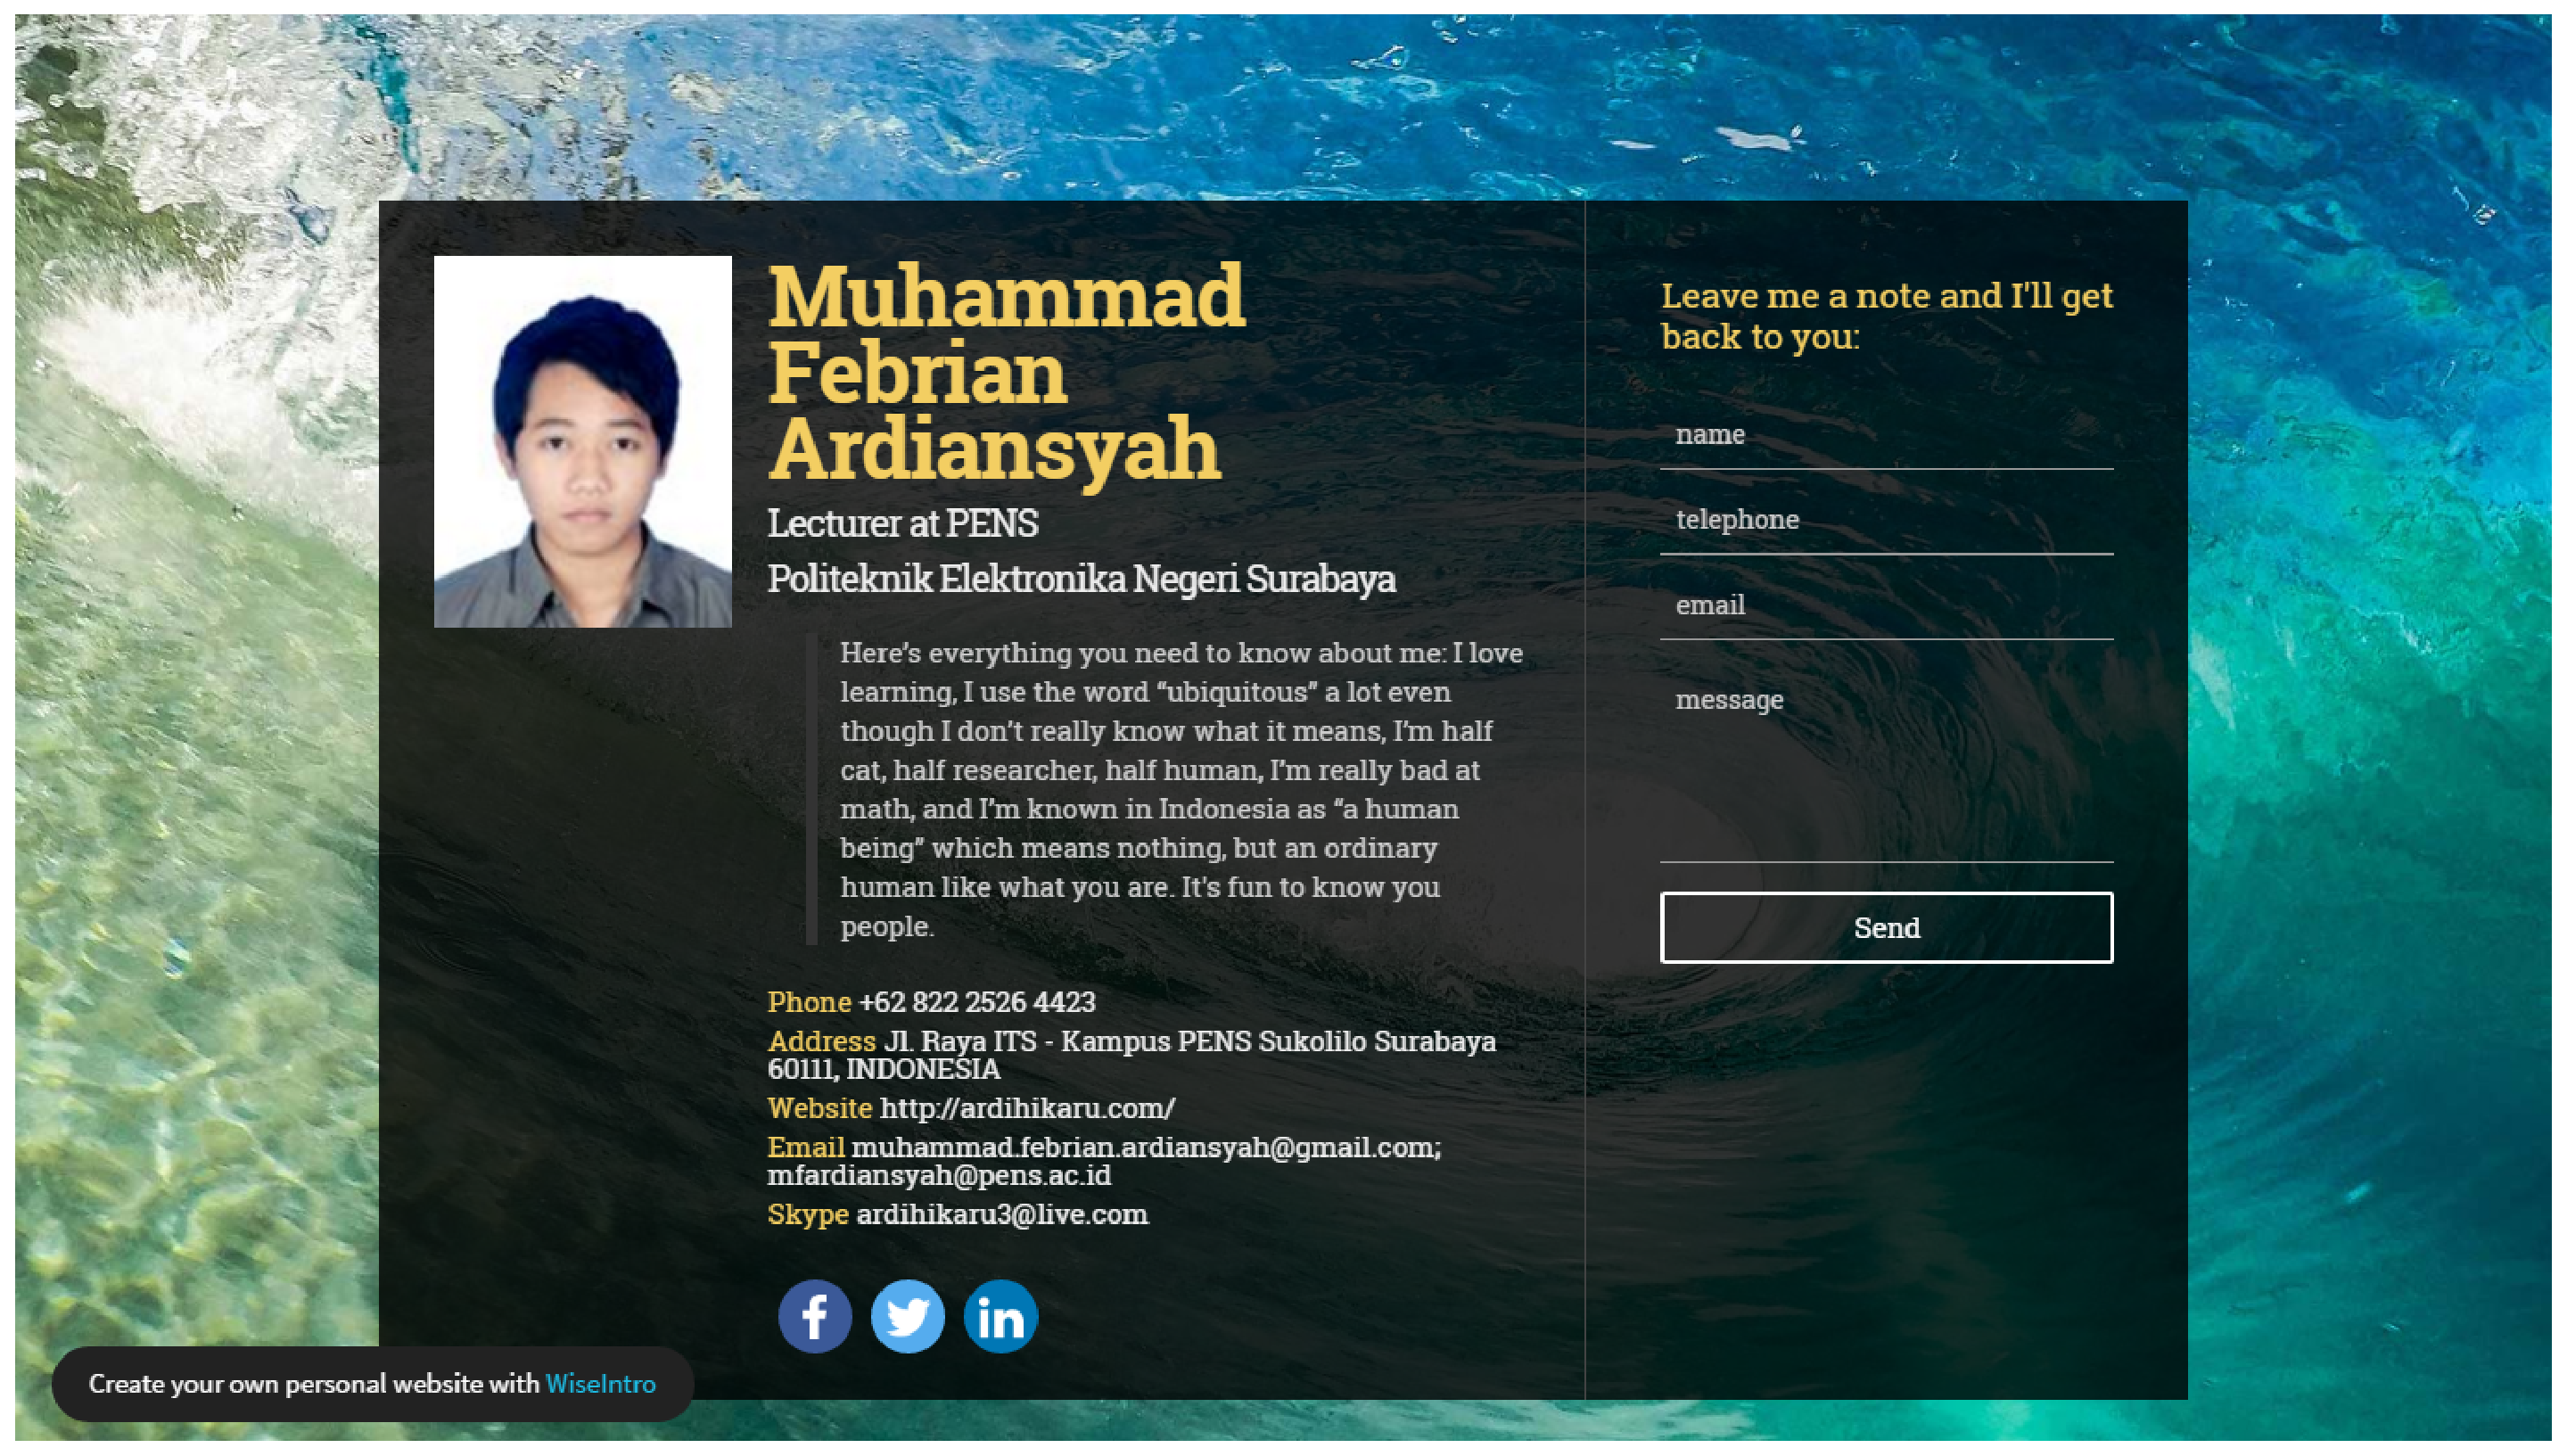
\includegraphics[width=120mm, height=120mm, keepaspectratio]{intro}
\caption{Intro}
\label{fig:fig1b}
\end{figure}

\section{Name of the section 1: e.g. Using figures}
Subsection is here. In latex, it is suggested to use $.eps$ extension as our figure files. Do not ask me why, just trust me, it works! haha. Saran saya, gunakanlah ekstensi $.eps$ untuk gambar-gambar anda. Jangan ditanya ya, percaya saja. (Why? Google it yourself!). 

I use this $online tool$ \footnote{\label{note:eps_converter1}\url{http://www.tlhiv.org/rast2vec/}}. to convert my images into EPS format (resulted smaller and acceptable size). However, sometimes the webpage went offline. If you find some alternative sites, please fell free to share with me, with us.

Use $\backslash ref\{fig:fig1a\}$ (example: Fig.~\ref{fig:fig1a}) to show a figure. In Fig.~\ref{fig:fig1a}, it gives an example of a figure with multiple subfigures. Name $fig:fig1a$ is taken from figure's label. Syntax $\backslash ref\{fig:fig1a\}$ digunakan untuk menampilkan gambar yang sudah di-$attach$ di paper ini. Gambar Fig.~\ref{fig:fig1a} mencontohkan sebuah gambar dengan beberapa sub-gambar.

\begin{figure}[H]
\centering
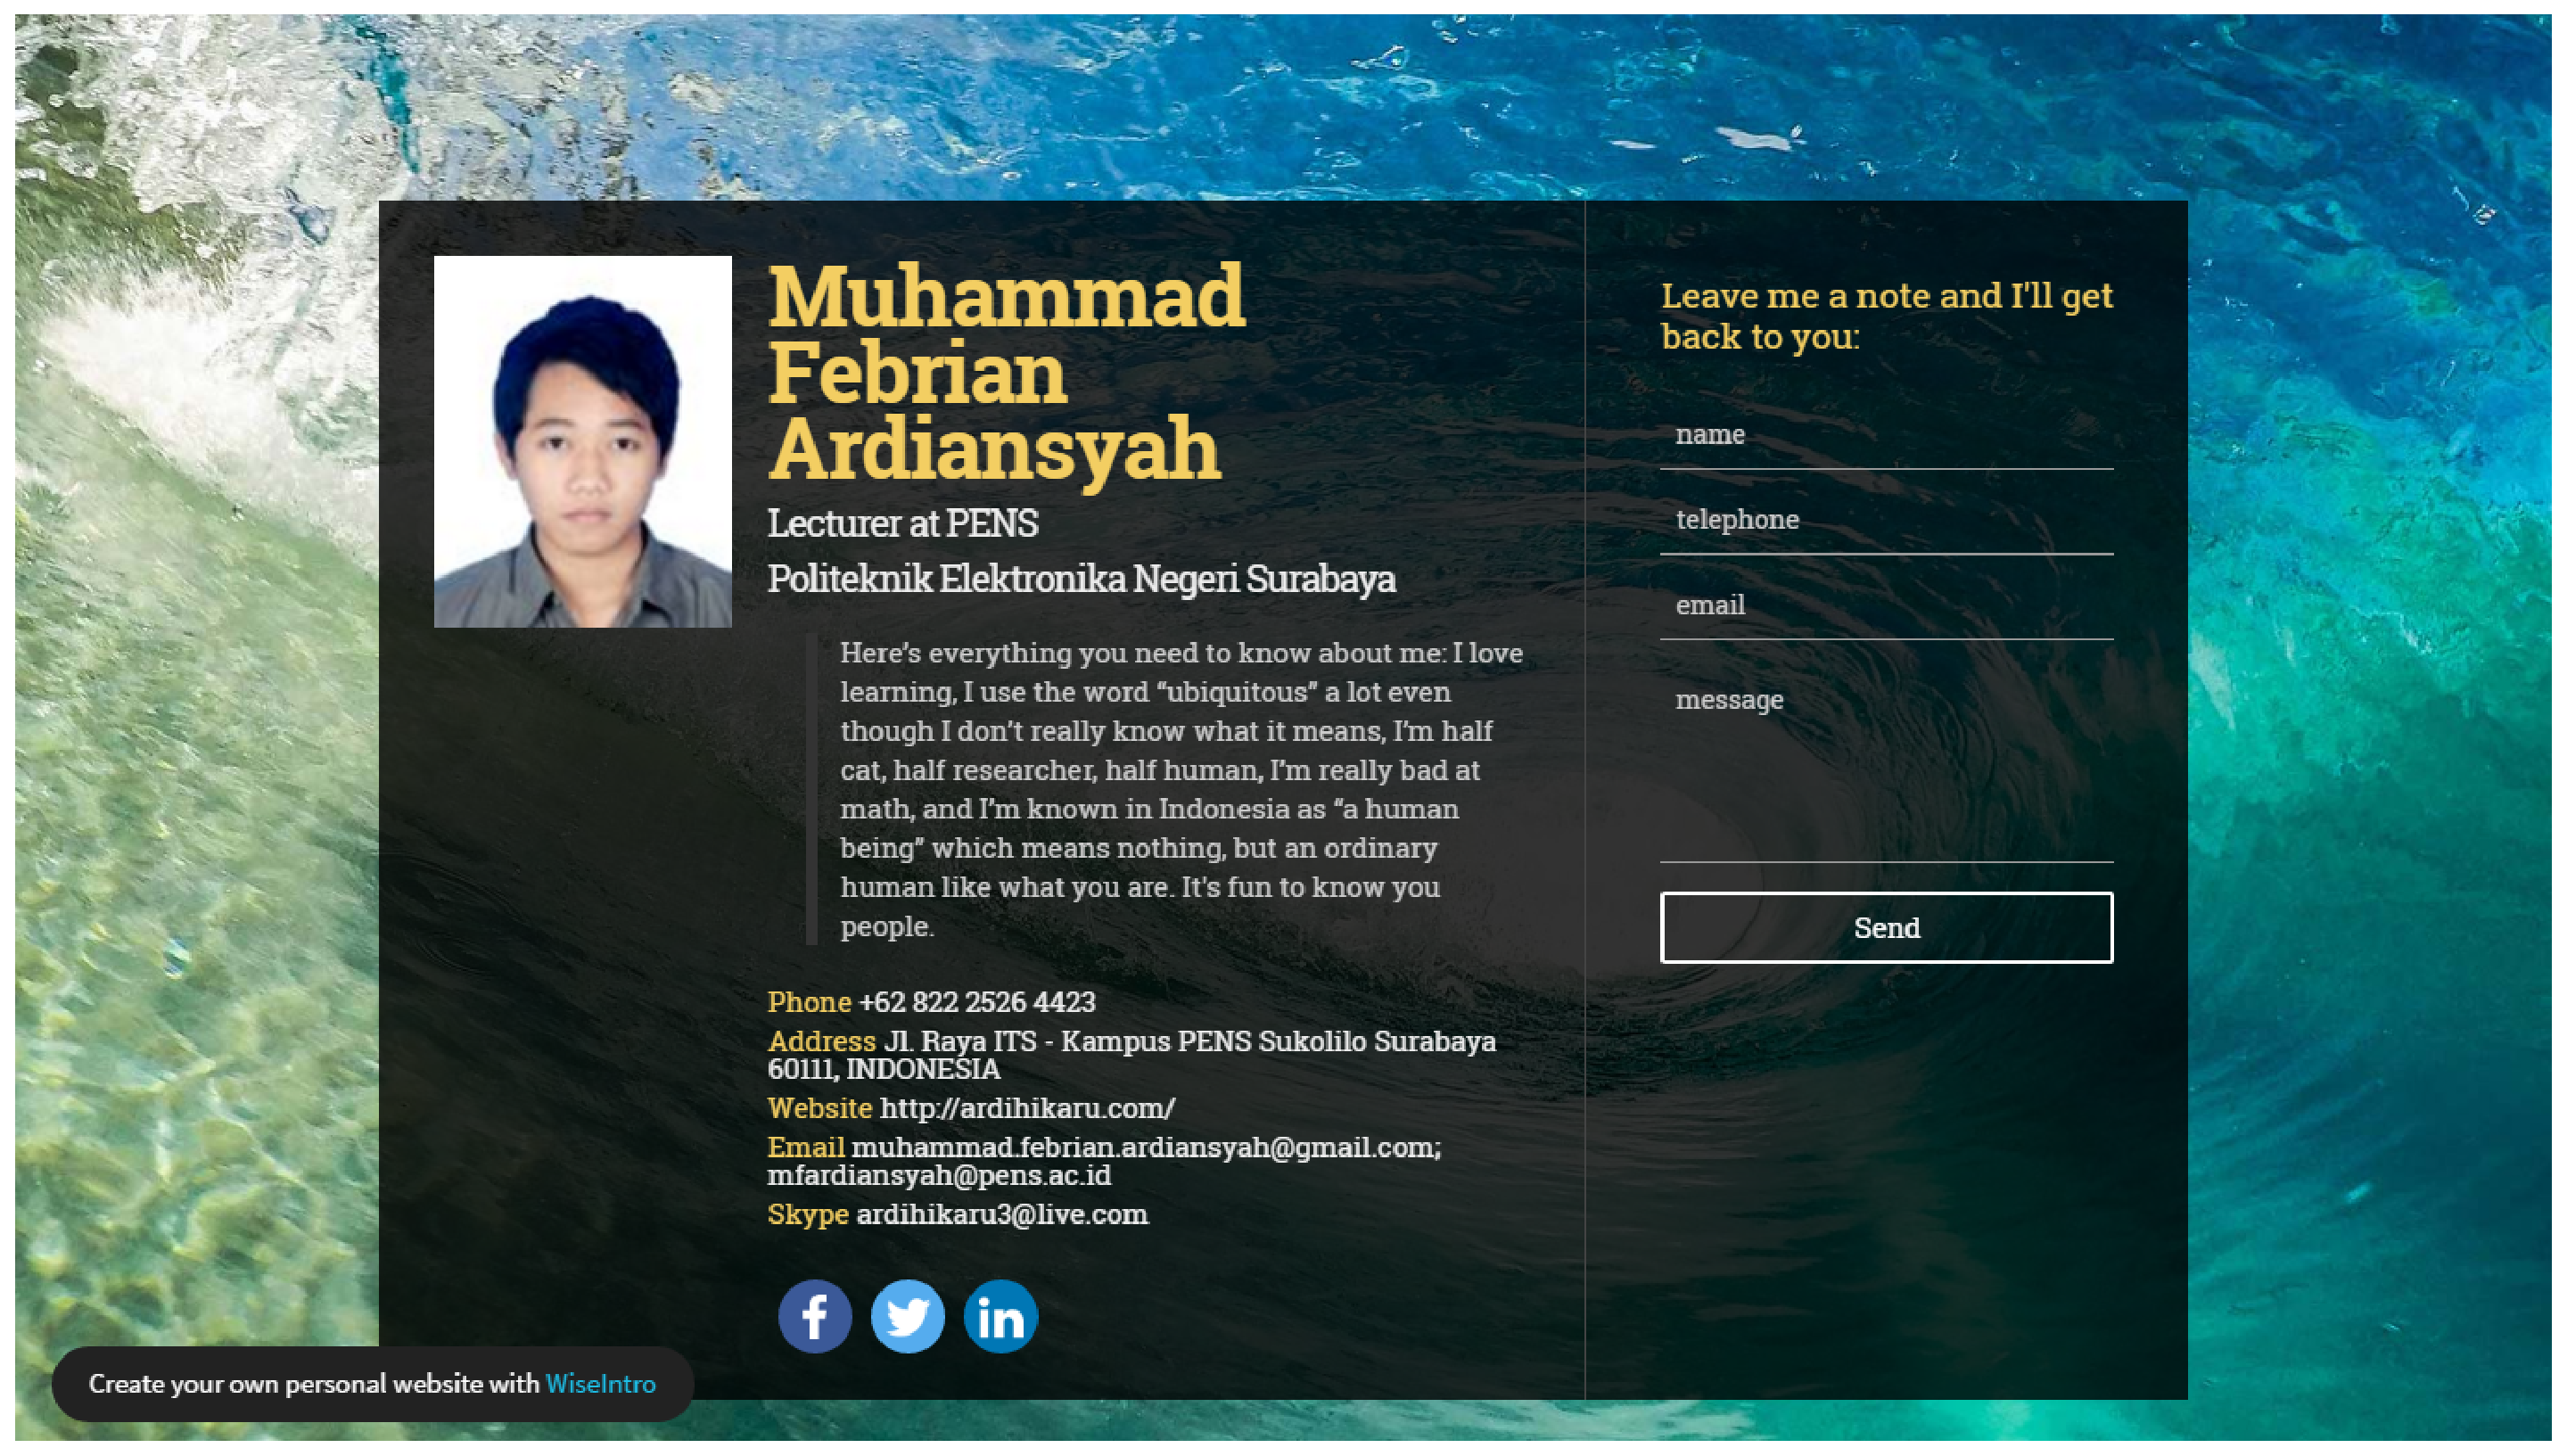
\includegraphics[width=120mm, height=120mm, keepaspectratio]{intro}
\caption{Intro}
\label{fig:fig2}
\end{figure}

Here is another way plot a figure. Fig.~\ref{fig:fig2} is a single figure. There are many ways to plot figures. For the further information, you can check it into $Latex \lq s~wiki$ \footnote{\label{note:latex_wiki_figures}\url{https://en.wikibooks.org/wiki/LaTeX/Floats,_Figures_and_Captions}}. Berikut merupakan cara lain untuk menampilkan gambar. Fig.~\ref{fig:fig2} adalah contoh untuk menampilkan sebuah gambar. Untuk informasi lebih detail, silahkan merujuk $Latex \lq s~wiki$ \footnotemark[\ref{note:latex_wiki_figures}] (yang ini menggunakan rujukan $footnote$). 

Here you may find this itemizing useful.
\begin{itemize}
  \item Item 1.
  \item Item 2.
  \item Item 3.
\end{itemize}

End of introduction section. You may close it with a summary like this: \textquote{\textit{In the rest of this paper, the related works are reviewed in Section 2. Our proposed architecture and system model is discussed in Section 3. Section 4 discusses the methodology we are using our proposed architecture. Then, Section 5 evaluates our research study with some simulation results. Finally, Section 6 summarizes this paper}}. Lanjuutttt...


